\documentclass[10pt,a4paper]{article}
\usepackage[utf8]{inputenc}
\usepackage[T1]{fontenc}
\usepackage[a4paper,top=1.5cm,bottom=1.5cm,left=1.5cm,right=1.5cm]{geometry}
\usepackage{amsmath}
\usepackage{amssymb}
\usepackage{tikz}
\usepackage{pgfplots}
\pgfplotsset{compat=1.18}
\pgfplotsset{
  grafik/.style={
    axis lines=middle,
    xlabel={$x$}, ylabel={$y$},
    width=7.5cm, height=6cm,
    grid=major, grid style={gray!25},
    tick label style={font=\scriptsize},
    every axis x label/.style={at={(ticklabel* cs:1)},anchor=west},
    every axis y label/.style={at={(ticklabel* cs:1)},anchor=south},
    title style={yshift=2ex},
  },
}
\usepackage[dvipsnames,svgnames]{xcolor}
\usepackage{booktabs}
\usepackage{tabularx}
\usepackage{array}
\usepackage[bookmarks=false]{hyperref}

\title{Rubrik Nilai Tugas Minggu 4 : Limit}
\author{Matematika untuk Sistem Informasi}
\date{}

\newenvironment{rubrik}{%
  \noindent
  \tabularx{\textwidth}{@{}>{\raggedright\arraybackslash}p{2.2cm}>{\raggedright\arraybackslash}X>{\centering\arraybackslash}p{1.1cm}>{\centering\arraybackslash}p{1.4cm}@{}}
  \toprule
  \textbf{Kriteria} & \textbf{Deskriptor} & \textbf{Maks} & \textbf{Skor} \\
  \midrule
}{%
  \bottomrule
  \endtabularx\par
}
\newcommand{\butir}[1]{\par\vspace{0.75em}\noindent\textbf{#1}\par\vspace{0.35em}}

\begin{document}
\maketitle

\noindent
Nama: \underline{\hspace{7.2cm}} \quad NIM: \underline{\hspace{4.2cm}}

\section*{Petunjuk penilai}
\begin{itemize}
  \item Tiap butir maksimum 100. Nilai tugas adalah rata-rata skor butir.
  \item Ketentuan skor:\par
  {\small
  \setlength{\tabcolsep}{4pt}%
  \begin{tabularx}{\linewidth}{@{}>{\raggedright\arraybackslash}p{2.1cm}>{\centering\arraybackslash}p{1.6cm}>{\raggedright\arraybackslash}X@{}}
  \toprule
  \textbf{Kriteria} & \textbf{Maks} & \textbf{Ketentuan} \\
  \midrule
  Langkah & 60 atau 70 & Jika langkah terbaca dan tidak seluruhnya salah, skor minimal 25. Skor di bawah 25 hanya bila langkah salah total, tidak dimengerti, atau tidak terbaca. \\
  Jawaban & 30 atau 40 & Harus ada dan benar. Skor hanya 0 atau nilai penuh. \\
  \bottomrule
  \end{tabularx}}
\end{itemize}

\butir{Butir 1(a). $\displaystyle\lim_{x \to -1}(1 - 2x)$ (100 poin)}
\begin{rubrik}
Langkah &
Fungsi polinom dikenali, lalu $x = -1$ disubstitusikan. &
70 & \\
Jawaban &
Limit sama dengan $3$. &
30 & \\
\midrule
\multicolumn{2}{r}{\textbf{Jumlah}} & 100 & \\
\end{rubrik}

\butir{Butir 1(b). $\displaystyle\lim_{t \to 3}\frac{t^2 + 4t - 21}{t - 3}$ (100 poin)}
\begin{rubrik}
Langkah &
Substitusi memberi $\frac{0}{0}$, lalu pembilang difaktorkan dan faktor yang sama dicoret. &
60 & \\
Jawaban &
Limit sama dengan $10$. &
40 & \\
\midrule
\multicolumn{2}{r}{\textbf{Jumlah}} & 100 & \\
\end{rubrik}

\butir{Butir 1(c). $\displaystyle\lim_{x \to 9}\frac{x - 9}{\sqrt{x} - 3}$ (100 poin)}
\begin{rubrik}
Langkah &
Bentuk $\frac{0}{0}$ dihilangkan dengan sekawan penyebut, lalu disubstitusi ulang. &
60 & \\
Jawaban &
Limit sama dengan $6$. &
40 & \\
\midrule
\multicolumn{2}{r}{\textbf{Jumlah}} & 100 & \\
\end{rubrik}

\butir{Butir 2. Membaca limit dan nilai fungsi dari grafik (100 poin)}
\begin{center}
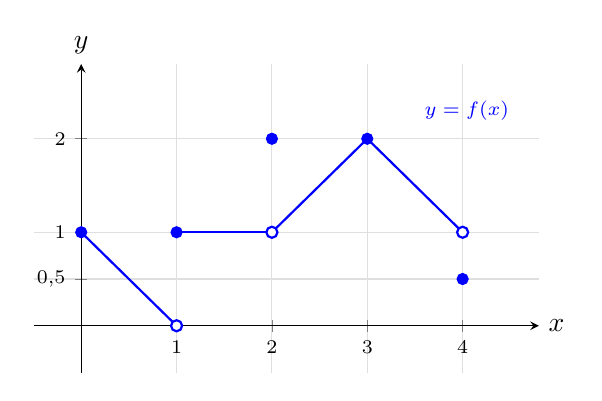
\begin{tikzpicture}
\begin{axis}[grafik, width=8cm, height=5.5cm, xmin=-0.5, xmax=4.8, ymin=-0.5, ymax=2.8,
  xtick={1,2,3,4}, ytick={0.5,1,2}, yticklabels={$0{,}5$,$1$,$2$}]
  \addplot[thick, blue, no marks] coordinates {(0,1) (1,0)};
  \addplot[thick, blue, no marks] coordinates {(1,1) (2,1)};
  \addplot[thick, blue, no marks] coordinates {(2,1) (3,2) (4,1)};
  \filldraw[blue] (axis cs:0,1) circle (2pt);
  \filldraw[blue, fill=white, thick] (axis cs:1,0) circle (2pt);
  \filldraw[blue] (axis cs:1,1) circle (2pt);
  \filldraw[blue, fill=white, thick] (axis cs:2,1) circle (2pt);
  \filldraw[blue] (axis cs:2,2) circle (2pt);
  \filldraw[blue] (axis cs:3,2) circle (2pt);
  \filldraw[blue, fill=white, thick] (axis cs:4,1) circle (2pt);
  \filldraw[blue] (axis cs:4,0.5) circle (2pt);
  \node[blue, font=\scriptsize, anchor=west] at (axis cs:3.5,2.3) {$y = f(x)$};
\end{axis}
\end{tikzpicture}
\end{center}
\begin{rubrik}
Langkah &
Limit dibaca dari arah kurva, nilai fungsi dari titik penuh; titik kosong tidak dipakai sebagai nilai fungsi. &
60 & \\
Jawaban &
(a)~$0$, (b)~$1$, (c)~$1$, (d)~$2$, (e)~tidak ada, (f)~$f(2)=2$, (g)~$f(3)=2$, (h)~$f(4)=0{,}5$. &
40 & \\
\midrule
\multicolumn{2}{r}{\textbf{Jumlah}} & 100 & \\
\end{rubrik}

\[
f(x) =
\begin{cases}
  x^2 + 1, & x \le 1 \\
  x^2 - x + 2, & x > 1
\end{cases}
\]
\butir{Butir 3(a). Limit kiri dan kanan $f$ di $x = 1$ (100 poin)}
\begin{rubrik}
Langkah &
Masing-masing sisi memakai aturan yang berlaku: $x^2+1$ dari kiri dan $x^2-x+2$ dari kanan. &
60 & \\
Jawaban &
$\lim_{x \to 1^-} f(x) = 2$ dan $\lim_{x \to 1^+} f(x) = 2$. &
40 & \\
\midrule
\multicolumn{2}{r}{\textbf{Jumlah}} & 100 & \\
\end{rubrik}

\butir{Butir 3(b). Keberadaan $\displaystyle\lim_{x \to 1} f(x)$ (100 poin)}
\begin{rubrik}
Langkah &
Limit dua sisi ada tepat jika limit kiri sama dengan limit kanan. &
60 & \\
Jawaban &
Limit ada dan nilainya $2$. &
40 & \\
\midrule
\multicolumn{2}{r}{\textbf{Jumlah}} & 100 & \\
\end{rubrik}

\butir{Butir 4(a). $\displaystyle\lim_{t \to 0}\frac{\sin 3t}{\tan t}$ (100 poin)}
\begin{rubrik}
Langkah &
Bentuk $\frac{0}{0}$ diubah ke pola $\frac{\sin u}{u}$. &
60 & \\
Jawaban &
Limit sama dengan $3$. &
40 & \\
\midrule
\multicolumn{2}{r}{\textbf{Jumlah}} & 100 & \\
\end{rubrik}

\butir{Butir 4(b). $\displaystyle\lim_{t \to 0}\frac{\sin^2 3t}{2t^2}$ (100 poin)}
\begin{rubrik}
Langkah &
Bentuk $\frac{0}{0}$ diubah ke kuadrat pola dasar sinus. &
60 & \\
Jawaban &
Limit sama dengan $\frac{9}{2}$. &
40 & \\
\midrule
\multicolumn{2}{r}{\textbf{Jumlah}} & 100 & \\
\end{rubrik}

\butir{Butir 4(c). $\displaystyle\lim_{x \to 0}\frac{3x \tan x}{\sin x}$ (100 poin)}
\begin{rubrik}
Langkah &
Identitas $\tan x = \frac{\sin x}{\cos x}$ dipakai sehingga faktor $\sin x$ tersederhanakan. &
60 & \\
Jawaban &
Limit sama dengan $0$. &
40 & \\
\midrule
\multicolumn{2}{r}{\textbf{Jumlah}} & 100 & \\
\end{rubrik}

\butir{Butir 5(a). $\displaystyle\lim_{n \to \infty}\frac{n^2}{2n + 1}$ (100 poin)}
\begin{rubrik}
Langkah &
Derajat pembilang lebih tinggi, atau pembagian dengan pangkat tertinggi penyebut. &
60 & \\
Jawaban &
Limit $+\infty$ (tidak ada sebagai bilangan real). &
40 & \\
\midrule
\multicolumn{2}{r}{\textbf{Jumlah}} & 100 & \\
\end{rubrik}

\butir{Butir 5(b). $\displaystyle\lim_{n \to \infty}\frac{3n^2}{2n^2 + 1}$ (100 poin)}
\begin{rubrik}
Langkah &
Derajat sama, pembagian dengan $n^2$. &
60 & \\
Jawaban &
Limit sama dengan $\frac{3}{2}$. &
40 & \\
\midrule
\multicolumn{2}{r}{\textbf{Jumlah}} & 100 & \\
\end{rubrik}

\butir{Butir 5(c). $\displaystyle\lim_{x \to \infty}\frac{x}{1 + x^2}$ (100 poin)}
\begin{rubrik}
Langkah &
Derajat penyebut lebih tinggi, pembagian dengan $x^2$. &
60 & \\
Jawaban &
Limit sama dengan $0$. &
40 & \\
\midrule
\multicolumn{2}{r}{\textbf{Jumlah}} & 100 & \\
\end{rubrik}

\section*{Rekap skor}
\noindent
\begin{tabular}{@{}lr@{}}
\toprule
Butir & Skor \\
\midrule
1(a) & \\
1(b) & \\
1(c) & \\
2 & \\
3(a) & \\
3(b) & \\
4(a) & \\
4(b) & \\
4(c) & \\
5(a) & \\
5(b) & \\
5(c) & \\
\midrule
Rata-rata = jumlah skor / 12 (maksimum 100) & \\
\bottomrule
\end{tabular}

\end{document}
